\documentclass[../Languages.tex]{subfiles}

\begin{document}
\usec{Python 3}\label{sec:python_3}

\cd{Python} is an interpreted high-level programming language for
general-purpose programming. Created by Guido van Rossum and first released in
1991, \cd{Python} was a esign philosophy that emphasized code readability, and
a syntax that allows programmers to express concepts in fewer lines of code,
notably using siginificant whitespae. It provides contructs that enable clear
programming on both small and large scales.

\cd{Python} features a dynamic type system and automatic memory management. It
supports multiple programming paradigms, including object-oriented, imperative,
functional and procedural, and has a large and comprehensive standard library.

\cd{Python} interpreters are available for many operating systems.
\cd{CPython}, the reference implementation of \cd{Python}, is open sourcce
software and has a community-based development model, as do nearly all of its
variant implmentations. \cd{CPython} is managed by the non-profit Python
Software Foundation.

\subsection{Influence}\label{sub:influence}

\begin{Figure}
  \centering
  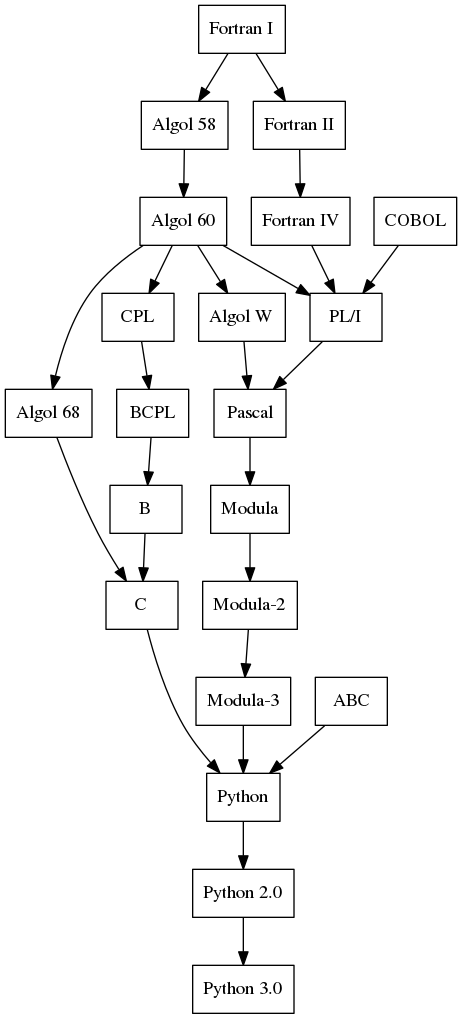
\includegraphics[height=0.5\textheight]{python3}
  \captionof{figure}{Inheritance diagram for \cd{Python 3}.}
\end{Figure}

\newpage
\end{document}
